\chapter{Virtualization and Containerization} \label{ch:vac}

Virtualization and containerization are widely appreciated technologies for distributing multiple instances of applications on single or multiple physical servers. The primary objective of these technologies is to enhance resource utilization efficiency while ensuring isolation between applications.

\section{Introduction}

One of the major differences between a server and a PC is that the former is usually shared among multiple users or applications at the same time. Though working on the same machine, a user would usually want a private working environment not interrupted by other users. In other words, a user would want to ``virtually'' work on an independent machine with his own CPU, RAM, I/O, OS, drivers and storage, despite that the actual hardware is shared with others. This can be achieved through \textit{virtualization}, which enables running multiple operating systems on a single physical server in an uninterrupted and logically separated manner. The virtually independent computer of such kind is often called a \textit{virtual machine} (VM).

Deploying a new VM generally consumes a considerably large amount of time and resources. This is because different VMs on the same server are separated at the OS level, with each VM requiring its own OS installation. Consider a scenario where there are hundreds of small applications (microservices), each requiring a similar but separate environment. Launching VMs for each and every of them is resource-intensive and can become an unnecessary waste of resource when these applications could have shared the same OS kernel and operated within their own isolated workspace.

A more efficient approach would be to deploy a single VM and place each application in a ``container'' with its own customized drivers and configurations. A container is similar to a VM in the sense that it provides a degree of isolation from others, but it is typically ``lighter'' than a VM because it doesn't need to virtualize or duplicate the whole OS as VMs do. This makes containers cheaper to launch and manage.

The technology used to deploy and manage containers is known as \textit{containerization}. A container contains all the configuration and requirement information of an application. Running a container on different platforms would consistently generate the same expected result. This has made the sharing and rapid deployment of containers remarkably easy and convenient. The similarities and differences of personal PCs, VMs, and container applications are summarized in Fig. \ref{ch:vac:fig:pcvmcontainersructure}.

\begin{figure}
	\centering
	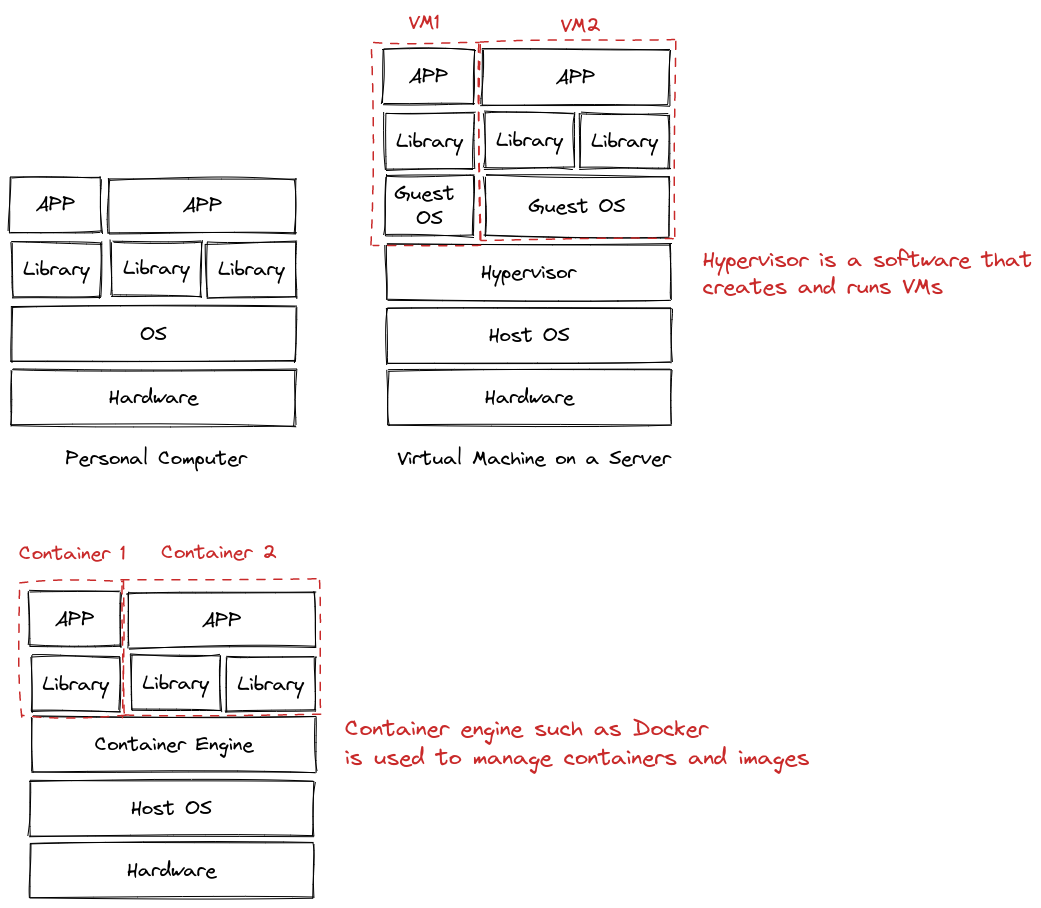
\includegraphics[width=350pt]{chapters/part-3/figures/pcvmcontainerstructure.png}
	\caption{System architectures of PC, VM and container.} \label{ch:vac:fig:pcvmcontainersructure}
\end{figure}

As an analogy, think of running an APP as asking a kitchen to prepare a dish. The hardware corresponds with the physical resources in the kitchen such as the cooktop and gas. The OS corresponds with the person who manages the kitchen, say a cook. The OS requires drivers and libraries to run the APP correctly. The drivers and libraries correspond with the skill sets or specific cookers for the dish. Finally, the APP is corresponding with the expected dish.

In the most simple configuration, a dedicated machine is used to run an APP. This is like constructing a dedicated kitchen and hiring a dedicated cook for each dish. The cook is trained to master all necessary skills required for that specific dish. This is shown in Fig. \ref{ch:vac:fig:acookinakitchen}.
\begin{figure}[htbp]
	\centering
	
\includegraphics[width=300pt]{chapters/part-3/figures/acookinakitchen.png}
	\caption{PC implementation: a cook in a kitchen.} \label{ch:vac:fig:acookinakitchen}
\end{figure}

In a VM implementation, a larger and more capable kitchen is setup in advance as shown in Fig. \ref{ch:vac:fig:manycooksinakitchen}. For each dish, a cook is hired. Each cook is trained with the skills necessary for his assigned dish. All cooks share the same kitchen. This implementation is more efficient than Fig. \ref{ch:vac:fig:acookinakitchen}, as there is no need to scale up the kitchen for a new dish. By sharing the resources among the cooks, the kitchen can be utilized more efficiently.
\begin{figure}[htbp]
	\centering 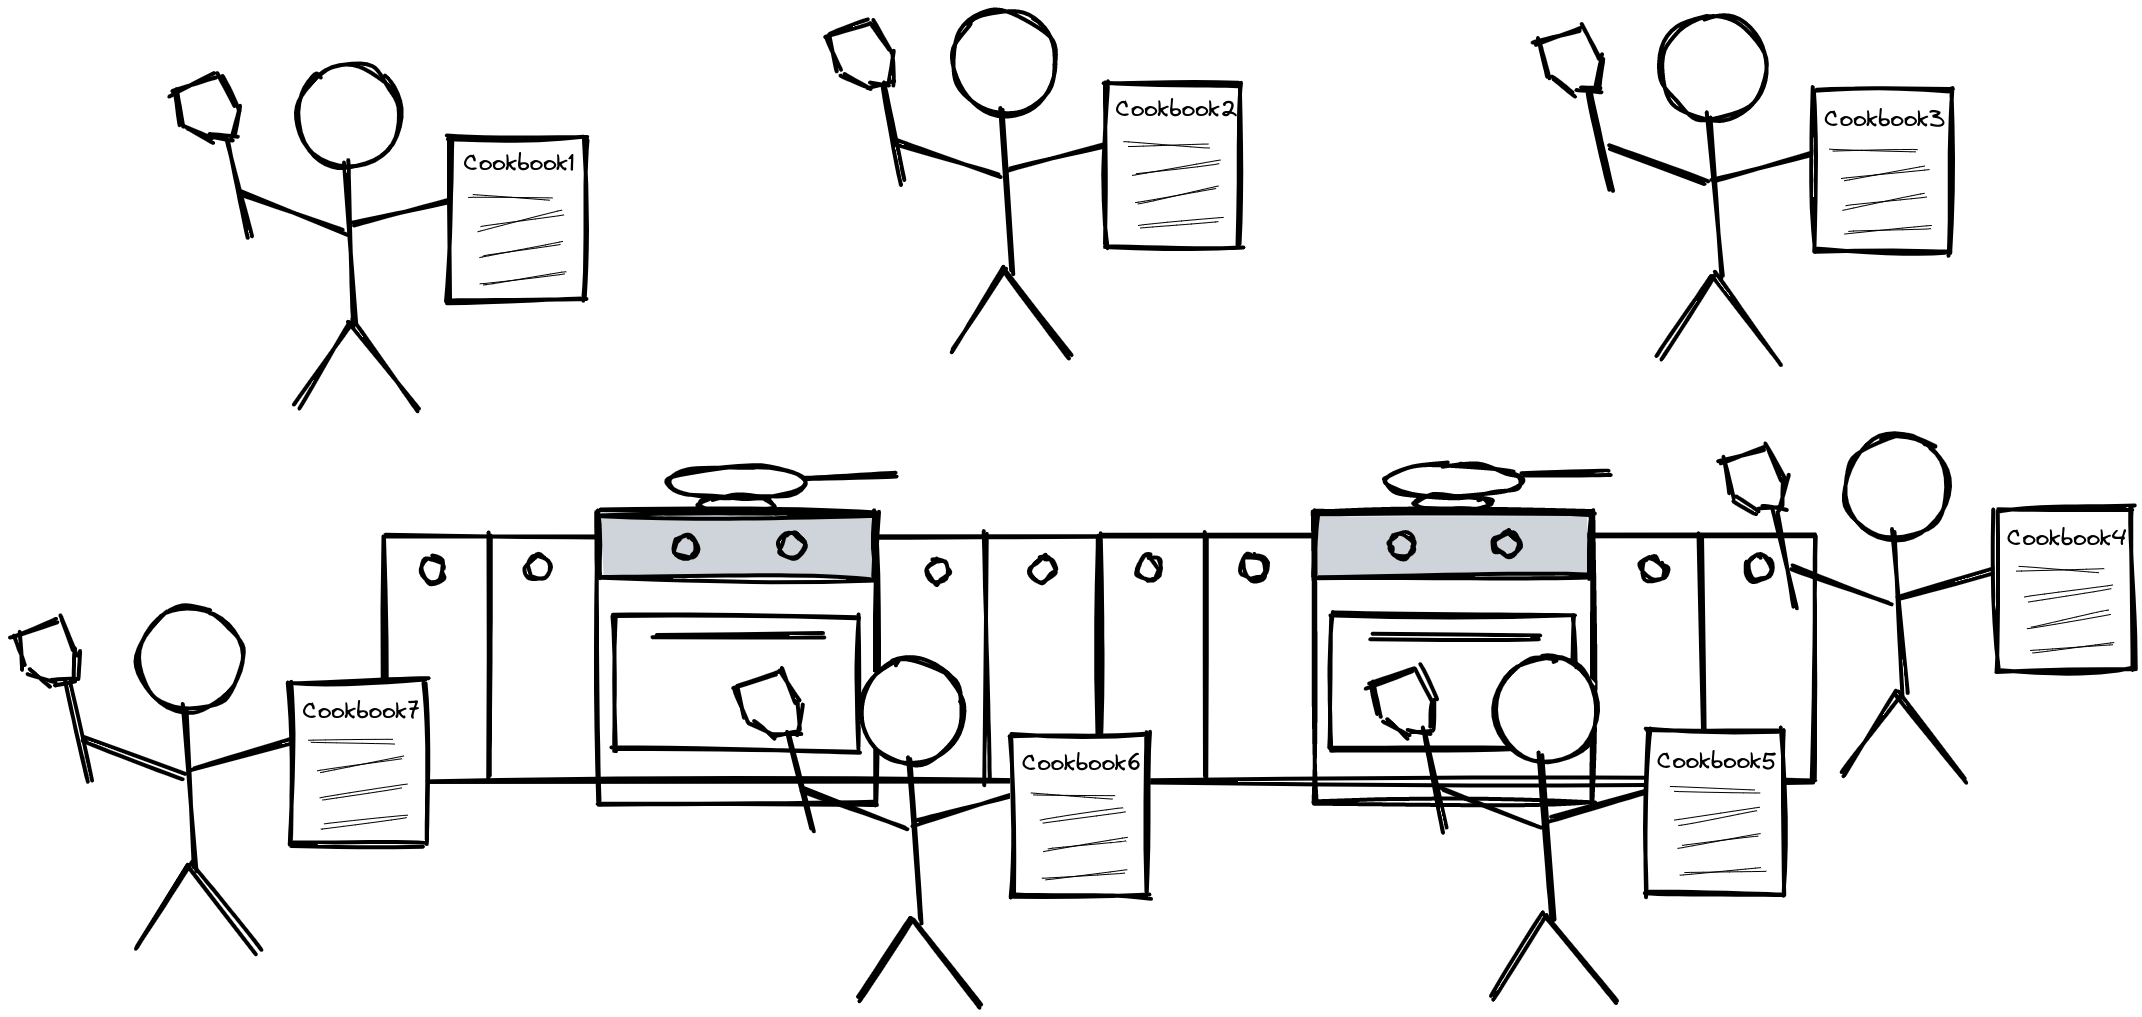
\includegraphics[width=350pt]{chapters/part-3/figures/manycooksinakitchen.png}
	\caption{VM implementation: many cooks in a kitchen, each with a different cookbook.} \label{ch:vac:fig:manycooksinakitchen}
\end{figure}

While Fig. \ref{ch:vac:fig:manycooksinakitchen} might be a popular practice in many restaurants, it is still too costly to hire a new cook for each dish. In a containerization implementation, a cook usually handles a category of dishes, as shown in Fig. \ref{ch:vac:fig:multitaskcook}. Of course, each dish will stay in its own fry-pan in an isolated way. For each dish, its receipt is provided that gives all information required to prepare the dish consistently. As long as the cook is good at multi-tasking, Fig. \ref{ch:vac:fig:multitaskcook} is usually a more efficient implementation than Figs. \ref{ch:vac:fig:acookinakitchen} and \ref{ch:vac:fig:manycooksinakitchen}.

\begin{figure}[htbp]
	\centering
	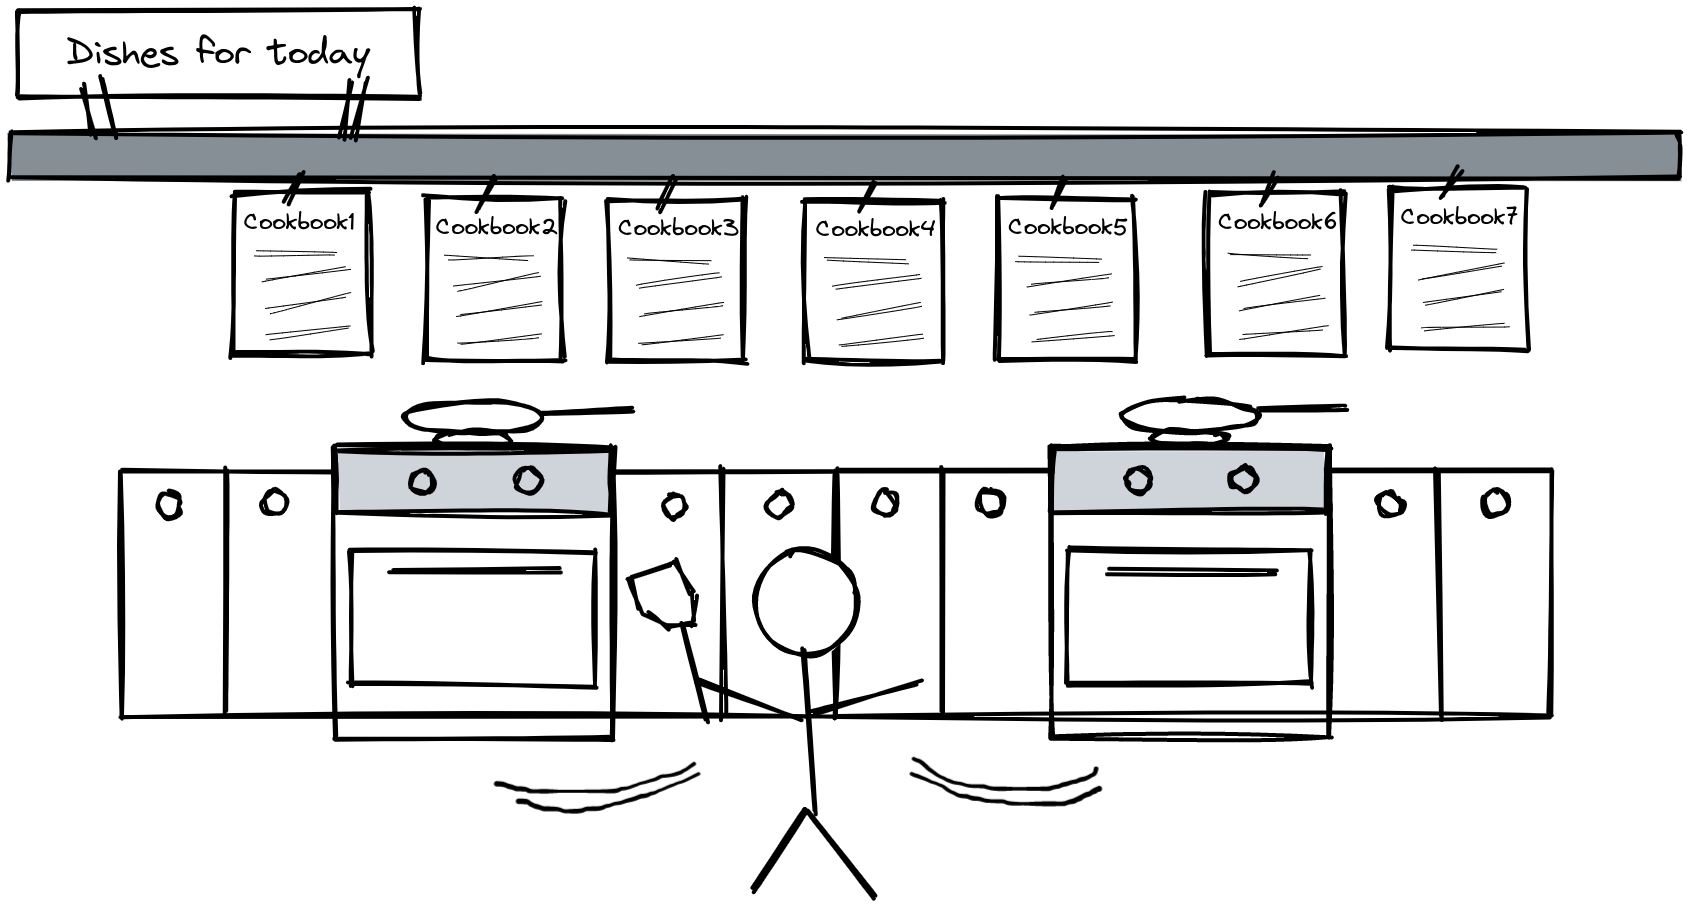
\includegraphics[width=350pt]{chapters/part-3/figures/multitaskcook.png}
	\caption{Container implementation: one cook in a kitchen, handling multiple dishes, each has a cookbook and stays in its own pan.} \label{ch:vac:fig:multitaskcook}
\end{figure}

Just like a receipt guaranteeing the consistency of dishes, in containerization, an ``image'' guarantees the consistent performance of container instances. An image is basically a collection of prerequisites and configurations to run a container quickly, efficiently and consistently. Images can be shared among machines to replicate the containers even if the machines adopt different underlying infrastructures such as hardware and OS.

\section{Virtualization and Containerization}

Virtualization and containerization have been studied for decades. This section gives a brief introduction to both technologies.

\subsection{Virtualization}

In a conventional data center, multiple physical servers are deployed, and each server has a single associated application. Servers may share the same LAN and network-attached storage (NAS) for data exchanging. A big issue of this implementation is the utilization efficiency of the servers and the unevenly distributed loads: some of the servers may not be utilized efficiently, while others may be overwhelmed. To deploy a new application, a new server must be purchased, which can take months of time. With more and more servers, the management and IT cost may grow exponentially.

To solve this problem, we need a systematical and automated way of integrating the resources in a data center and re-distributed them to the applications in an efficient manner. Virtualization is one of the most important technology used in this framework. Virtualization is essentially about running a system on a ``virtualized machine'', where by saying ``virtualized'' we mean that the machine is not a physical machine, but a running environment (known as the virtual execution environment) that is emulated and managed by a special software running on the actual machine (known as the ``hypervisor''). The setup should be transparent to the applications in the sense that the applications the same way as if it were running on a dedicated physical machine.

Depending on the items to be virtualized, virtualization can be divided into the following categories.
\begin{itemize}
  \item Virtualization of equipment, mainly network resources and storage. This results in virtual local area network (VLAN), virtual private network (VPN), NAS and storage area network (SAN).
  \item Virtualization of operating system. This results in the well-known VM and virtual desktop.
  \item Virtualization of application running environment. An example is Java virtual machine (JVM) that allows Java to generate consistent result while running on different machines.
\end{itemize}

There are different virtualization architectures. Widely seen components in the virtualization architectures include
\begin{itemize}
	\item Host OS. The OS that resides on the physical machine, on which virtualization tools run.
	\item Virtual Machine Monitor (VMM), also known as the hypervisor. This is a software that runs on the host OS, managing all the guest OS, providing them interface to the host OS and the hardware.
	\item VM, a virtual system that runs in an virtualized isolated environment.
\end{itemize}
Host OS, VMM and VM relationship is shown in Fig. \ref{ch:vac:fig:acookinakitchen}.

Different virtualization techniques are used in different types of VMMs. They can be widely divided into the following categories.
\begin{itemize}
	\item Full virtualization. The VMM virtualizes everything including the hardware. The guest OS can run on the VM without modification or adaptation, just like running on any other machine.
	\item Paravirtualization. The VMM does not virtualize hardware. The guest OS is modified to certain extent to suit the VMM of this type.
	\item Hardware-assisted virtualization. The physical processors provide some specific services to handle some of the functionality of VMM. Some functions requested by the guest OS, after passing to VMM, is directly run on the hardware, thus enhancing system performance.
\end{itemize}

VMM is able to virtualize hardware resources such as CPU, memory and I/O. For the virtualization of CPU, the key is to virtualize privileged instructions (a set of instructions that can only be executed by software running in privileged mode, usually the OS) for the guest OS, so that the guest OS would think it is directly talking to a CPU. This is challenging because guest OS usually does not possess the privilege due to the VM architecture. If the requests of the guest OS contain privileged instructions, the CPU will deny the instructions. When that happens, an exception will be raised to the VMM which will take care of the privileged instructions sequentially. Since hypervisor runs in privileged mode, it can execute those instructions.

For the virtualization of memory, VMM uses shadow page table to assign memory pages to different VMs. The maximum memory allocated to a VM can change dynamically.

For the virtualization of I/O, the development trend is that I/O operations will be less and less rely on software and OS, and more and more on hardware. The VMM directly maps the I/O hardware interface to the VMs.

\begin{shortbox}
	\Boxhead{Hypervisor VS Host OS, Who is the Boss?}
	Both the hypervisor and the host OS can run in privilege mode (also known as ``Ring 0'' in x86 architecture). However, notice that at one time there can be only one boss, i.e., there can be only one entity that runs in Ring 0 at the same time.
	
	Depending on the type of the hypervisor configuration, this entity can be either the hypervisor or the host OS. In a type 1 hypervisor configuration, the hypervisor itself runs in Ring 0 and manages all hardware resources directly. In a type 2 hypervisor configuration, the host OS runs in Ring 0, and the hypervisor runs in a lower privileged ring.
\end{shortbox}

\subsection{Containerization}

Containerization is an alternative virtualization approach to VM that can also virtualize an independent workspace for an application. Comparing with VM, containers are often lighter, hence more efficient for massive microservices deployment. Depending on the context, the term ``container'' may refer to one or more of the following 3 components: container runtime, container engine, and container orchestration.

Container runtime refers to the backend software that actually runs the containers, and it is compulsory for all types of container implementation. Examples of widely used container runtimes are ``containerd'', ``runc'' and ``cri-o''. It is often inconvenient for users to talk to container runtimes directly. Container engine is the interface for a user or software to manage images and containers. Examples of container engines include ``docker'' and ``podman''. Finally, container orchestration is the software that strategically deploy, monitor, restart, and terminate the containers on servers. It can scale up and down the number of containers based on the demanding, and balance the API calls each container receives. Container orchestration is very useful in production environment of a large service. One of the most widely used container orchestrations is ``kubernetes''.

Notice that container orchestration may or may not bypass the container engine and talk to the container runtime directly.

\section{Docker Container} \label{ch:vac:sec:dc}

This section introduces docker. Notice that although docker is famous for docker container engine, docker as a company or community provides many revolutionary container related tools and services that go far beyond a container engine brand. Many tools and technologies of docker are used in container runtimes and container engines of other brands.

This section focuses mostly on the introduction of docker container engine.

\subsection{Docker Engine VS Alternatives}

Docker engine is the most popular container engines available on the market as of 2023, and it is free of charge for open-source, personal and small business usage. More details of docker can be found at \textit{https://docs.docker.com/}.

But does that mean docker engine is the absolutely best and perfect container engine solution?

Docker has surely revolutionized how we use containerization technology in software development and deployment, and it has been one of the most popular and beloved container engine solutions. However, it is worth mentioning that docker engine is not the only available container engine. For example, as explained earlier podman is an alternative to docker. It supports the same interface as docker in its CLI (as if podman were an alias), and claims to have better performance and security. As a matter of fact, RHEL already started the transition from docker to podman from RHEL 8. Nowadays, installing docker on the latest versions of RHEL is possible but tedious. On the other hand, installation of podman on RHEL, if it had not been pre-installed, can be done simply by
\begin{lstlisting}
$ sudo dnf install podman
\end{lstlisting}
Kubernetes, a famous container orchestration, is also dropping docker support according to their statement ``docker support in the kubernetes is now deprecated and will be removed in a future release''. Some may even argue that ``containers are alive, but the role that docker plays is shrinking''. Many open-source initiatives such as podman are gaining popularity.

Docker has some disadvantages indeed. For one thing, docker uses docker server (docker daemon), a single piece of software running in the backend of the system, to support all the services. This creates a single-point-of-failure in the system. Docker requires root privileges, and it starts a container on behalf of the root user. This means that the program running inside the container and the users in the docker group can potentially bypass the OS access control and gain root access, which introduces security risk. These shortages are to some extent addressed by other container engines such as podman which is daemon-less and does not necessarily need to run on root user's behalf.

This is not to say that Docker is falling behind as a whole. Some key techniques that docker introduced are widely used in all different types and brands of container runtimes and engines. It is just that people do not like some of the features of docker engine, and alternative tools are being developed to fix these problems, the latter of which starting drawing more and more attention. Docker still enjoys widespread usage and support due to its massive community, wealth of online resources, and extensive compatibility with numerous tools and platforms. Nevertheless, for demonstration purpose, for the remaining sections docker is used throughout this notebook. Since podman provides the same interface, it is probable that podman can be used likewise to replicate all the results.

As of 2023, docker is still the dominating container market engine, with a market share of over $80\%$.

\subsection{Docker Installation}

To install docker on a Linux machine, go to \textit{https://www.docker.com/} to look for the instruction. The installation steps differ depending on the host machine. As an example, consider installing docker engine on Ubuntu. Some of the key steps are summarized as follows.

Remove existing docker engine, if any.
\begin{lstlisting}
$ sudo apt-get remove docker docker-engine docker.io
$ sudo apt-get remove containerd runc
\end{lstlisting}
Add docker's official GPG key and set up the repository.
\begin{lstlisting}
$ sudo apt-get update
$ sudo apt-get install ca-certificates curl gnupg lsb-release
$ sudo mkdir -p /etc/apt/keyrings
$ curl -fsSL https://download.docker.com/linux/ubuntu/gpg | sudo gpg --dearmor -o /etc/apt/keyrings/docker.gpg
$ echo \
  "deb [arch=$(dpkg --print-architecture) signed-by=/etc/apt/keyrings/docker.gpg] https://download.docker.com/linux/ubuntu \
  $(lsb_release -cs) stable" | sudo tee /etc/apt/sources.list.d/docker.list > /dev/null
\end{lstlisting}
Install docker.
\begin{lstlisting}
$ sudo apt-get update
$ sudo apt-get install docker-ce docker-ce-cli containerd.io docker-compose-plugin
\end{lstlisting}
To test whether docker is installed correctly, run
\begin{lstlisting}
$ sudo docker run hello-world
\end{lstlisting}
and if everything is done correctly, a message started with ``Hello from Docker!'' will be displayed in the console, together with a brief introduction to how docker works.

Notice that to use docker commands, sudo privilege is required. To avoid typing \verb|sudo| each time running a docker command, add the user to the docker group as follows. In the rest of the section, \verb|sudo| is neglected for docker commands.
\begin{lstlisting}
$ sudo usermod <user name> -aG docker
\end{lstlisting}

Docker installs at least two piece of software on the machine, namely docker CLI and docker server. The CLI is the interface to the user, and the server is the actual tool that manages images and containers. Docker runs natively on Linux OS. If docker is installed on non-Linux system such as Windows or macOS, ``docker desktop'' is used which includes a Linux VM to host the docker daemon and run Linux-based containers.

\subsection{Docker Container Management}

\vspace{0.1in}
\noindent \textbf{Container Manipulation}
\vspace{0.1in}

To create and run a container from an image, simply use
\begin{lstlisting}
$ docker run <configuration> <image>
\end{lstlisting}
which is a combination of \verb|docker create| and \verb|docker start|. Docker will search the local and remote repositories for the image, download the image if necessary, and start a container from that image. By default, after successful execution and completion of all the tasks, the container will enter ``Exited'' status. For example, consider running a container of \textit{alpine} as follows. A screen shot is given in Fig. \ref{ch:vac:fig:dockerrunexp}.
\begin{lstlisting}
$ docker run -it --name test-alpine alpine
\end{lstlisting}
where \verb|-i| stands for ``interactive'', which keeps the container's standard input (i.e., the console in this example) open so that the user can actively interact with the container. Option \verb|-t| allocates a pseudo-TTY to the container. TTY stands for ``TeleTYpewriter'', which enforces the I/O of the container to follow the typical terminal format and allows the user to interact with the container like a traditional terminal, hence making the interactive interface a bit more user-friendly. Finally, \verb|--name| assigns a name to the container. Without an assigned name, docker will assign a random name to the container.
\begin{figure}[htbp]
	\centering
	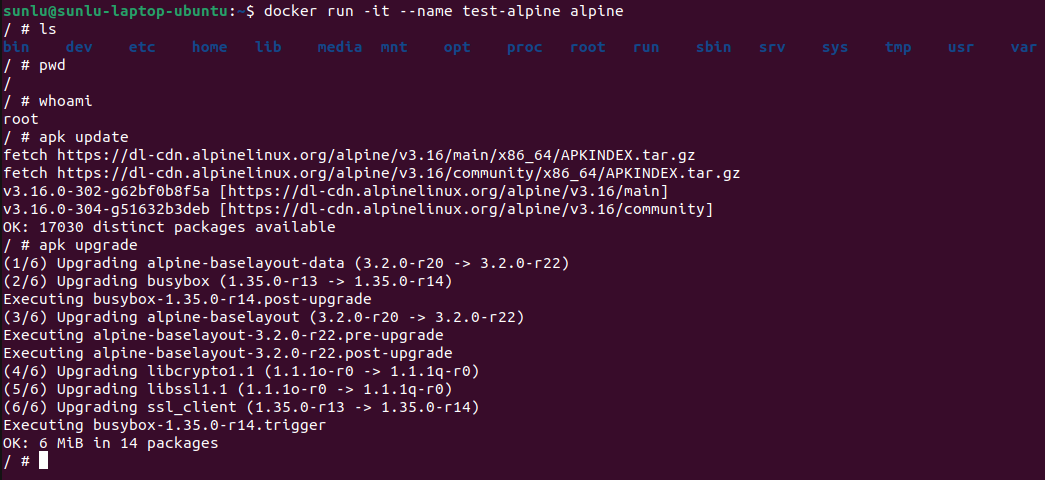
\includegraphics[width=350pt]{chapters/part-3/figures/dockerrunexp.png}
	\caption{An example of running \textit{apline} container, with interactive TTY and name \textit{test-apline}.} \label{ch:vac:fig:dockerrunexp}
\end{figure}

It can be seen from Fig. \ref{ch:vac:fig:dockerrunexp} that once the container is started, the user can interact with the container via shell, and perform actions such as listing items in the current directory in the container. While keeping the container running, open another terminal and use \verb|docker container ls|. The container \verb|test-alpine| shall appear in the list, as shown in Fig. \ref{ch:vac:fig:dockerrunexppart2}.
\begin{figure}[htbp]
	\centering
	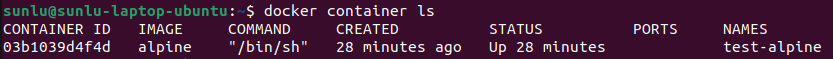
\includegraphics[width=250pt]{chapters/part-3/figures/dockerrunexppart2.png}
	\caption{List the running container \textit{test-apline}.} \label{ch:vac:fig:dockerrunexppart2}
\end{figure}
After exiting from Fig. \ref{ch:vac:fig:dockerrunexp} (by using \verb|exit| in \textit{alpine}), the container will transfer its status from ``running'' to ``exited'', as shown in Fig. \ref{ch:vac:fig:dockerrunexppart3}.
\begin{figure}[htbp]
	\centering
	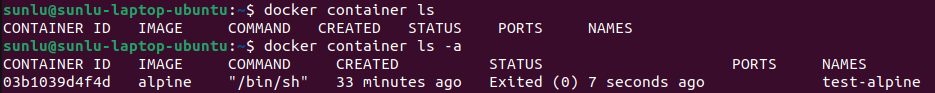
\includegraphics[width=250pt]{chapters/part-3/figures/dockerrunexppart3.png}
	\caption{List the exited container \textit{test-apline}.} \label{ch:vac:fig:dockerrunexppart3}
\end{figure}

As introduced earlier, \verb|docker run| contains two consecutive steps in the backend, namely \verb|docker create| and \verb|docker start|, where \verb|docker create| creates a container, with all its file system setup, and \verb|docker start| starts the container by executing the startup script defined in the image. These two commands can be used separately. For example, to start an exited container, use
\begin{lstlisting}
$ docker start <container>
\end{lstlisting}
This command starts the container with the startup command, and keep it running in the backend. If \verb|-a| is used in front of the container id, the container's IO would be attached to the terminal. If the startup command has been overwritten during the creation of the container, the new startup command will be used. The container id and the revised startup command can be obtained using \verb|docker container ls -a|.

It is also possible to launch a container and let it run in the backend using \verb|-d| flag which stands for ``detached mode''. An example is given below.
\begin{lstlisting}
$ docker run -dt --name test-background-alpine alpine
\end{lstlisting}
By changing \verb|-i| to \verb|-d|, the container runs in the backend silently. The status of the container, after executing the above command, will stay running and can be displayed by \verb|docker container ls|.

Commonly used commands regarding launching a container are given in Tables \ref{ch:vac:tab:launchcontainer}, and \ref{ch:vac:tab:listcontainer}.

\begin{table}
	\centering \caption{Commonly used docker commands to launch a container.}\label{ch:vac:tab:launchcontainer}
	\begin{tabularx}{\textwidth}{llX}
		\hline
		Command & Flag & Description \\ \hline
		\verb|docker run| & --- & Launch a container of the image. If the image cannot be found locally, it downloads the image from the remote repository automatically. \\ 
        \verb|docker run| & \verb|-i| & Keep the standard input of the container open when launching the container. \\ 
        \verb|docker run| & \verb|-d| & Launch the container in the backend and keep it running. \\ 
        \verb|docker run| & \verb|--rm| & Automatically remove the container when exiting. The removed container will not be listed in \verb|docker container ls -a|. This is usually used with temporary containers during debugging. \\ 
        \verb|docker run| & \verb|-t| & Allocate a pseudo-TTY. The flag usually comes with the flags \verb|-i| or \verb|-d|, to form \verb|-it| or \verb|-dt|. \\ 
        \verb|docker run| & \verb|--restart| & Enforce restart of the container upon exiting. This is usually used on containers running in the backend. Commonly used restart configurations include \verb|--restart no| (do not restart), \verb|--restart on-failure[:<max retries>]| (restart if exits with an error flag), \verb|--restart always| (always restart when exists). \\ 
        \verb|docker run| & \verb|--name| & Assign a name to the container. \\
		\hline
	\end{tabularx}
\end{table}

\begin{table}
	\centering \caption{Commonly used docker commands to display local images and containers.}\label{ch:vac:tab:listcontainer}
	\begin{tabularx}{\textwidth}{llX}
		\hline
		Command & Flag & Description \\ \hline
        \verb|docker image ls| & --- & List local images. \\ 
        \verb|docker container ls| & --- & List running containers. \\ 
        \verb|docker container ls| & \verb|-a| & List all containers. \\
		\hline
	\end{tabularx}
\end{table}

It is worth mentioning that file system snapshot and startup commands are defined inside an image. See Section \ref{ch:vac:sec:di} for more details. When a container starts, the file system snapshot is pasted to the container file system, and the startup commands executed. It is possible to overwrite the startup commands when starting a container, simply by amending the revised startup commands to the image name as follows.
\begin{lstlisting}
$ docker run <image> <revised command>
\end{lstlisting}
where \verb|<revised command>| must be defined in the image, or otherwise an error will be raised.

For a container running in the backend, use \verb|docker exec| to execute a shell command in that container as follows.
\begin{lstlisting}
$ docker exec <container> <command>
\end{lstlisting}
To enable the TTY shell of a container running in the backend, use
\begin{lstlisting}
$ docker exec -it <container> <command>
\end{lstlisting}
If \verb|<command>| is replaced by the shell name used in the container, this would open the terminal of the container. Notice that the shell used by the application running inside the container may differ from the one used in the host machine. In the case of an \textit{alpine} image based container, \verb|ash| is the default shell. For a \textit{ubuntu} image based container, \verb|bash| is often used. To exit from the TTY shell while keep the container running in the backend, use shortcut key \verb|Ctrl+p+q|. An alternative way to interact with containers running in the backend is to use
\begin{lstlisting}
$ docker attach <container>
\end{lstlisting}
to attach local standard input, output, and error streams to a running container. Similar with the previously introduced \texttt{docker exec -it} command, \texttt{docker attach} also starts the shell of the application running in the container. Use \verb|Ctrl-C| to quite the shell.

To stop, kill or restart a container running in the backend, use
\begin{lstlisting}
$ docker stop <container>
$ docker kill <container>
$ docker restart <container>
\end{lstlisting}
respectively. The difference between \verb|docker stop| and \verb|docker kill| concerns with how the OS manages process. When \verb|docker stop| is used, a  \verb|SIGTERM| signal is sent to the main process that the container runs. The container still has a little bit of time (maximum $10$ seconds) to terminate the job and clean up. When \verb|docker kill| is used, \verb|SIGKILL| signal is sent to the process, and the process is terminated immediately. When a container is stopped, it enters exited status.

To remove an exited container or all exited containers, use
\begin{lstlisting}
$ docker container rm <container>
\end{lstlisting}
or
\begin{lstlisting}
$ docker container prune
\end{lstlisting}
respectively. Notice that there is a more powerful command
\begin{lstlisting}
$ docker system prune
\end{lstlisting}
which removes not only stopped containers but also unused network configurations, dangling images and cache.

To rename a container (without changing its container ID or anything else), use
\begin{lstlisting}
$ docker rename <container-old-name> <container-new-name>
\end{lstlisting}

\vspace{0.1in}
\noindent \textbf{Container Monitoring}
\vspace{0.1in}

Use
\begin{lstlisting}
$ docker container ls
\end{lstlisting}
to check the list of running containers, and
\begin{lstlisting}
$ docker container ls -a
\end{lstlisting}
the list of all containers, running or exited. Alternatively, \verb|docker ps|, \verb|docker ps -a| can also be used to list down containers just like \verb|docker container ls|, \verb|docker container ls -a|.

To check the processes that is running in the container, use
\begin{lstlisting}
$ docker top <container>
\end{lstlisting}

To quickly check container status including resource consumption (CPU, memory usage, etc.), use
\begin{lstlisting}
$ docker stats [<container>]
\end{lstlisting}
where the user can choose to list down all containers or a specified container. To show more detailed information of a container, including its status, gateway, IP address, etc., use
\begin{lstlisting}
$ docker inspect <container>
\end{lstlisting}
Finally, to check the logs of a container (e.g., its standard output to the console), use
\begin{lstlisting}
$ docker logs <container>
\end{lstlisting}

\vspace{0.1in}
\noindent \textbf{File Exchange between Container and Host Machine}
\vspace{0.1in}

There are multiple ways and protocols to access the files in a container, depending on the I/O setup of the container. For a container running locally, \verb|docker cp| can be used for file transfer between the container and the host machine as follows. From container to host machine:
\begin{lstlisting}
$ docker cp <container>:<source> <destination>
\end{lstlisting}
and from host machine to container:
\begin{lstlisting}
$ docker cp <source> <container>:<destination>
\end{lstlisting}
where \verb|<source>| and \verb|<destination>| refer to the path to the source and destination, respectively, located in the host machine or the container.

\vspace{0.1in}
\noindent \textbf{Commit Container to Image}
\vspace{0.1in}

A container is usually generated from an image. It is also possible to do vise versa, i.e., packaging a container into an image. Notice that this is generally not recommended. Images shall be created mostly from Dockerfile, as will be introduced in Section \ref{ch:vac:sec:di}.

To create an image from a container, use
\begin{lstlisting}
$ docker commit <container> <image>
\end{lstlisting}
or
\begin{lstlisting}
$ docker commit -c 'CMD ["<startup command>"]' <container> <image>
\end{lstlisting}
where \verb|docker commit| command saves the container's file changes or settings into a new image, which allows easier populating containers or debugging in a later stage. Notice that \verb|docker commit| does not save everything of the container into the image, and it is not the only way an image is created.

\vspace{0.1in}
\noindent \textbf{Publish Ports}
\vspace{0.1in}

By default, containers do not expose any ports to the outside world. A container can be accessed only from its host machine using APIs provided by docker, such as \verb|docker cp| to transfer files and \verb|docker exec| to execute commands, but not network protocols. The user can allow public access from the internet by publishing the ports of the container using
\begin{lstlisting}
$ docker run -p <host machine port>:<container port> <image>
\end{lstlisting}
when starting a container. To publish multiple ports, use multiple \verb|-p| flags in a command.

In a typical web service application, the host machine and the containers are often designed following the architecture similar with Fig. \ref{ch:vac:fig:containerwebserverarchitecture}. Notice that in practice, the load balancer and the containers may or may not run on the same physical machine.

The load balancer is a container orchestration that monitors the status of the containers, manages the data flow, and scales up and down the number of containers depending on the total load. In case where there are multiple physical servers, the load balancer is run on a ``master'' server, and the containers are distributed on multiple ``slave'' servers, each of which is called a ``worker node'', or ``node'' for simplicity. Container engines are installed on each and every node. The load balancer talks with the container engines on each node to deploy containers. The APP instances shall run in the containers distributively.
\begin{figure}[htbp]
	\centering
	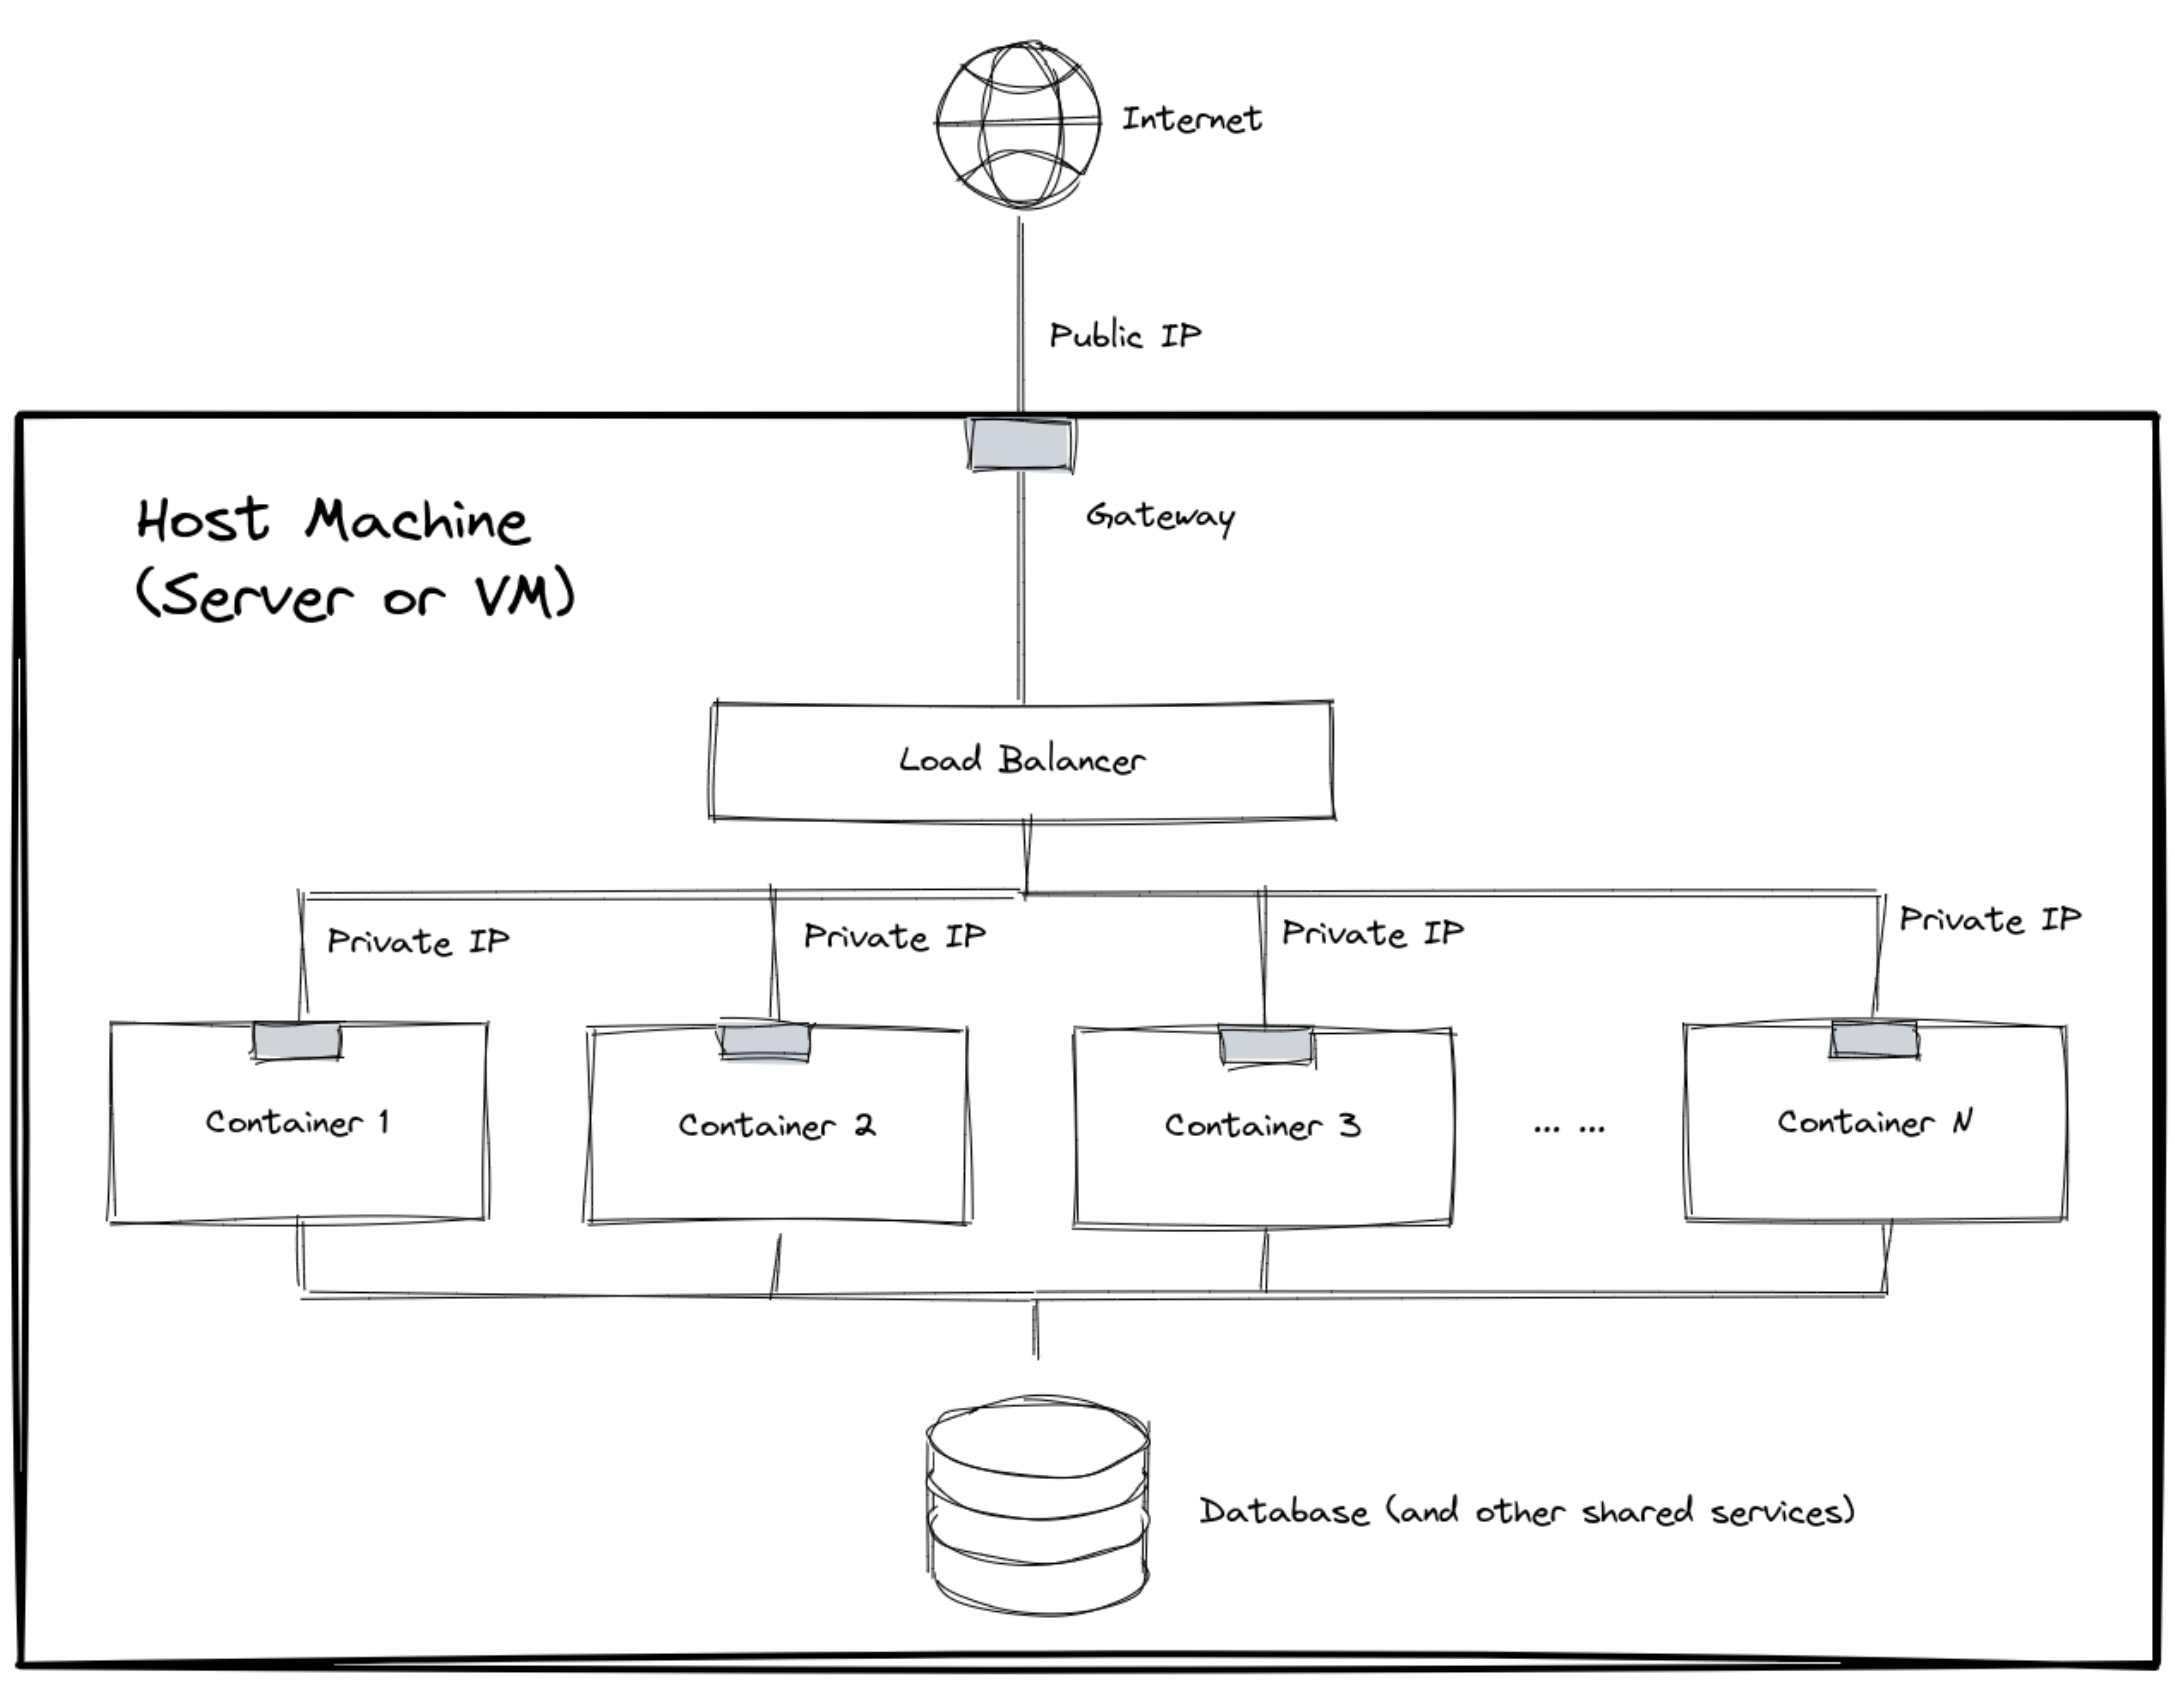
\includegraphics[width=350pt]{chapters/part-3/figures/containerwebserverarchitecture.png}
	\caption{A simplified architecture where containers are used to host the web service.} \label{ch:vac:fig:containerwebserverarchitecture}
\end{figure}

More about container orchestration is introduced in a later section.

\subsection{An Example}

An example of setting up a web server in containers from scratch is given in this section. For simplicity, everything happens on a single physical server. Only one container is used and the load balancer and the shared services are not included in the example.

As a first step, create a container from the official \textit{nginx} image as follows. Notice that it is also possible to create a container from \textit{apline}, and install \textit{nginx} on \textit{apline}.
\begin{lstlisting}
$ docker run -dt --name simple-web nginx
\end{lstlisting}

Next, create the configuration file for \textit{nginx}, and also the \textit{html} files to be used as the static web page. For convenience, the files are created and edited in the host machine, then copied to the container. The following \textit{default.conf} and \textit{index.html} have been created, respectively. The configuration file \textit{default.conf} is given below.
\begin{lstlisting}
server {
	listen 80 default_server;
	listen [::]:80 default_server;
	root /var/www/html/;
}
\end{lstlisting}
The \textit{html} file \textit{index.html} is given below.
\begin{lstlisting}
<html>
	<body>
		<h1>Hello World!</h1>
	</body>
</html>
\end{lstlisting}
Use \verb|docker copy| to copy the two files to the designed locations in the container as follows.
\begin{lstlisting}
$ docker exec simple-web mkdir -p /var/www/html
$ docker cp default.conf simple-web:/etc/nginx/conf.d/default.conf
$ docker cp index.html simple-web:/var/www/html/index.html
\end{lstlisting}
where \verb|mkdir -p| creates the directories along the given path, if not exist. Notice that the file name in the destination can be ignored if it is the same with the source, i.e., the copy commands can be replaced by
\begin{lstlisting}
$ docker cp default.conf simple-web:/etc/nginx/conf.d/
$ docker cp index.html simple-web:/var/www/html/
\end{lstlisting}

Change the ownership of the \textit{html} file as follows, so that the current user \textit{nginx} is able to access that file.
\begin{lstlisting}
$ docker exec simple-web chown -R nginx:nginx /var/www/html
\end{lstlisting}

Finally, reload and configuration file and restart the web server as follows.
\begin{lstlisting}
$ docker exec simple-web nginx -s reload
\end{lstlisting}

To test the web server running inside the container, obtain the IP address of the container using
\begin{lstlisting}
$ docker inspect simple-web | grep IPAddress
\end{lstlisting}
and open a browser to key in the obtained IP address. If everything is done correctly, the browser should try to access port 80 of the container, and the ``Hello World!'' web page shall show up.

For easy sharing and populating of the container, commit the container into a new image using \verb|docker commit| as follows. The new image can be used to populate the web server, just like ``web01'' container given below.
\begin{lstlisting}
$ docker commit simple-web simple-web-image
$ docker run -dt --name web01 -p 80:80 simple-web-image
\end{lstlisting}
where \verb|-p <host machine port>:<container port>| is used to map ports. Notice that different from the previous container ``\textit{simple-web}'', the new container ``\textit{web01}'' IP address port 80 is mapped with the port 80 of the host machine. Therefore, the web page hosted in ``\textit{web01}'' can be accessed not only by the host machine, but also by other machines in the same network with the host machine.

\section{Docker Volume} \label{ch:vac:subsec:dockervolume}

As introduced earlier, \verb|docker cp| can be used to transfer data into and out of a container. An alternative way of accessing docker container data from the host machine is to use docker volume. Docker volume is used to mount host machine hard drive to container storage. Details are introduced below.

To create a docker volume, use
\begin{lstlisting}
$ docker volume create <volume>
\end{lstlisting}
To list down volumes and to inspect a volume, use
\begin{lstlisting}
$ docker volume ls
$ docker volume inspect <volume>
\end{lstlisting}
respectively. Finally to remove a volume or all volumes, use
\begin{lstlisting}
$ docker volume rm <volume>
$ docker volume prune
\end{lstlisting}
respectively.

When starting a container from an image, volumes can be mapped with the internal storage inside the container by using \verb|-v| flag as follows
\begin{lstlisting}
$ docker run -v <volume>:<container-internal-path>[:ro] <image>
\end{lstlisting}
which should mount \verb|<volumn>| to \verb|<container internal path>|. The optional \verb|:ro| can be specified if it is a read-only volume. Instead of using a volume name, the path to a directory in the host machine can also be used, in which case the specified directories in the host machine and in the container should be synchronized.

Docker volume guarantees data persistence in containerized applications. When a docker container is removed, any data written to the container's writable layer is lost. Docker volumes, however, are stored outside of the container's writable layer, allowing data to persist even after the container is removed. This persistence is particularly important for applications that require permanent storage, such as databases.

Moreover, docker volumes can be shared among multiple containers, which facilitates data exchange and allows containers to work on the same dataset. Therefore, docker volumes are not just a tool for data persistence, but also an effective mechanism for data sharing and collaboration among containers.

The data persists in the docker host, and from the container's perspective, it is treated as a mounted volume. Hence, the data is not duplicated physically.


\section{Docker Image} \label{ch:vac:sec:di}

Container image related operations are introduced in this section.

\subsection{Docker Image Creation from Dockerfile}

Images are used to create containers. An image performs like a blueprint that encapsulates all the necessary information needed to spawn a container. It includes initial configurations, requisite libraries, and other pertinent metadata. Docker images are highly portable and can be shared across various machines and platforms. This section delves deeper into the construction and functionality of docker images.

An image shall contain everything needed to create and initialize a container. This includes but not limited to:
\begin{itemize}
  \item Necessary steps to create a container
  \item Files to support the application
  \item Libraries, tools and dependencies
\end{itemize}
In addition, an image shall be designed and organized in such a way that it is migratable, reusable and light, and can be used to easily populate large number of containers. For better inheritability, an image might be based on another existing image, which is called its parent image. An image with no parent, such as the official \textit{hello-world} image from docker bub, is called a base image.

The Dockerfile is a text document that serves as the blueprint for constructing a docker image. Generally speaking, a Dockerfile follows the following flow:
\begin{enumerate}[(1)]
	\item Specify base image
	\item Add additional configurations
	\begin{itemize}
		\item Setup file system
		\item Install dependencies and other programs
		\item Setup working directory
		\item Handle access control
		\item ...
	\end{itemize}
	\item Specify startup command
\end{enumerate}
A more detailed step-by-step guidance example is given later. The relationship between Dockerfile, image and container is illustrated in Fig. \ref{ch:vac:fig:dockerfiletoimage}. Notably, the Dockerfile itself isn't included within the resulting image.

\begin{figure}[htbp]
	\centering
	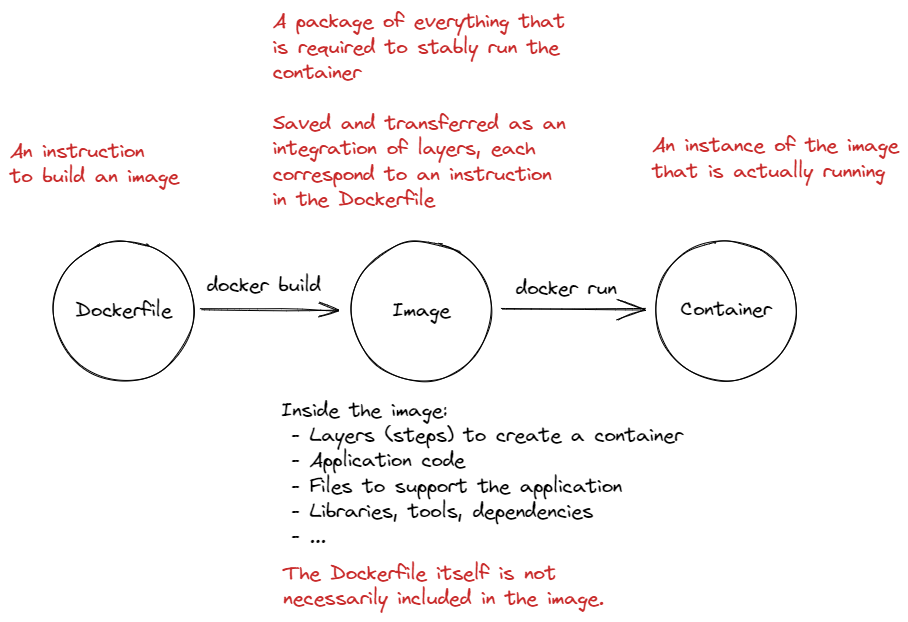
\includegraphics[width=350pt]{chapters/part-3/figures/dockerfiletoimage.png}
	\caption{A demonstration of how Dockerfile, image and container link to each other.} \label{ch:vac:fig:dockerfiletoimage}
\end{figure}

Since a docker image's primary role is to serve as a template for containers, many Dockerfile commands appear like a ``step-by-step'' recipe for container creation. Each instruction corresponds to an ``image layer''. An image is, in essence, an amalgamation of these layers. It is stored and distributed in this format. If images share layers (for instance, different versions of the same app), these shared layers are not saved or transferred redundantly, hence significantly reducing image sizes. More details can be found at \textit{https://docs.docker.com/storage/storagedriver/}.

Docker containers employ a special file system known as the Union File System (UFS), which is well suited to the ``layer'' concept. UFS facilitates file sharing between the container and the host machine, along with combining read-only upper layers and writable lower layers, among other functions. A demonstration to illustrate this concept is given later in Fig. \ref{ch:vac:fig:dockerlayerdemo}.

Just as a quick example, the Dockerfile to build the official \textit{hello-world} image from docker hub looks like the following.
\begin{lstlisting}
FROM scratch
COPY hello /
CMD ["/hello"]
\end{lstlisting}
Like other computer languages, Dockerfiles have reserved keywords, environment variables, and syntax rules. Only the basics of constructing a Dockerfile are introduced in this section. More details can be found in the Docker reference on the official website. In the example above, \verb|FROM scratch| signifies that this image is a base image without a parent. The \verb|COPY hello /| instruction copies the \textit{hello} binary script from the image to the root directory of the container. Lastly, \verb|CMD ["/hello"]| runs the \textit{hello} binary script.

In general, a typical Dockerfile includes the following instructions to build an image. These instructions allow the image to know how to create a container, automatically construct the file system directory structure, install necessary packages, and run the app:
\begin{enumerate}[(1)]
  \item Define parent image.
  \item Create filesystem directory.
  \item Set working directory.
  \item Copy files.
  \item Configure registry.
  \item Install packages.
  \item Copy more files after package installation.
  \item Switch to the correct user.
  \item Expose port.
  \item Run the application.
\end{enumerate}

The keywords to be used in a Dockerfile to realize the above instructions, such as \verb|FROM|, \verb|RUN|, and many more, are explained in Table \ref{ch:vac:tab:keywordsdockerfile}.

\begin{table}
	\centering \caption{Critical keywords used in a Dockerfile.}\label{ch:vac:tab:keywordsdockerfile}
	\begin{tabularx}{\textwidth}{lX}
		\hline
		Syntax & Description \\ \hline
		\verb|FROM <image>| & Define the parent image. A Dockerfile must start with a \verb|FROM| instruction. A Dockerfile can contain multiple \verb|FROM| instructions, in which case the last \verb|FROM| statement is the final base image and the earlier \verb|FROM| instructions creates intermediate images that can be used in the final image. An optional \verb|:<tag>| following \verb|<image>| can be used to specify the version of the image to use as the base. By default, the latest version of the image is used. \\ 
		\verb|RUN <command>| & Execute a shell command using \verb|/bin/sh -c|. \\ 
		\verb|WORKDIR <path>| & Set the working directory from the point onward. This prepares the working directory for the upcoming \verb|RUN|, \verb|COPY|, etc., commands. \\ 
		\verb|ADD <src> <dest>| & Add (Copy) \verb|<src>|, either a directory/file or URL, to \verb|<dest>|. An optional \verb|[--chown=<user>:<group>]| can be used to specify the owner and group of the added files. \\ 
		\verb|COPY <src> <dest>| & Copy \verb|<src>|, a directory/file, to \verb|<dest>|. An optional \verb|[--chown=<user>:<group>]| can be used to specify the owner and group of the added files. Notice that \verb|COPY| is similar with \verb|ADD|. \verb|COPY| is easier but less powerful than \verb|ADD|. It cannot handle tar or URL. \\ 
		\verb|USER <user>| & Switch user for the instructions beyond this point. \\ 
		\verb|EXPOSE <port>| & Specifies the ports that the container shall listen to. An optional \verb|/<protocol>| following \verb|<port>| can be used to specify the protocol for communication. \\ 
		\verb|CMD ["<exe>", "p1", ...]| & The user-script command. This is the last instruction in the docker file that usually starts the APP. Notice that a Dockerfile can only contain one \verb|CMD| instruction. The executable command name and the parameters are put into a list. This user-script can be overwritten by \texttt{docker run <image> <other commands>} when running the container. \\
		\hline
	\end{tabularx}
\end{table}

Besides Table \ref{ch:vac:tab:keywordsdockerfile}, there are other Dockerfile keywords that can significantly simplify the design and maintenance of the image. For example, \verb|ENV <key>=<value>| assign a value to an environmental variable; \verb|LABEL <key>="<value>"| assigns a tag to the image, which can be displayed when \verb|docker inspect <container>| is used.

Examples of Dockerfiles are given below, one from \textit{docs.docker.com} and the other from Linux Academy. The docker image layer structure of the second example is given in Fig. \ref{ch:vac:fig:dockerlayerdemo} as a demonstration. Notice that in Fig. \ref{ch:vac:fig:dockerlayerdemo}, \verb|bootfs| refers to the ``boot file system'', including the bootloader and the Linux kernel. Upon run, a container layer will be added to the image, as shown by the blue dashed box in Fig. \ref{ch:vac:fig:dockerlayerdemo}. In the container, all the changes made is saved into the container layer.

To generate a new image to include the changes made in the container, use \verb|docker commit|, which essentially commits the container layer as the latest image layer in the new image, as shown by the green dashed box in Fig. \ref{ch:vac:fig:dockerlayerdemo}.

\begin{lstlisting}
# First Example
FROM golang:1.16
WORKDIR /go/src/github.com/alexellis/href-counter/
RUN go get -d -v golang.org/x/net/html
COPY app.go ./
RUN CGO_ENABLED=0 GOOS=linux go build -a -installsuffix cgo -o app .

FROM alpine:latest
RUN apk --no-cache add ca-certificates
WORKDIR /root/
COPY --from=0 /go/src/github.com/alexellis/href-counter/app ./
CMD ["./app"]
\end{lstlisting}

\begin{lstlisting}
# Second Example
FROM node:10-alpine
RUN mkdir -p /home/node/app/node_modules && chown -R node:node /home/node/app
WORKDIR /home/node/app
COPY package*.json ./
RUN npm config set registry http://registry.npmjs.org/
RUN npm install
COPY --chown=node:node . .
USER node
EXPOSE 8080
CMD ["node", "index.js"]
\end{lstlisting}

\begin{figure}[htbp]
	\centering
	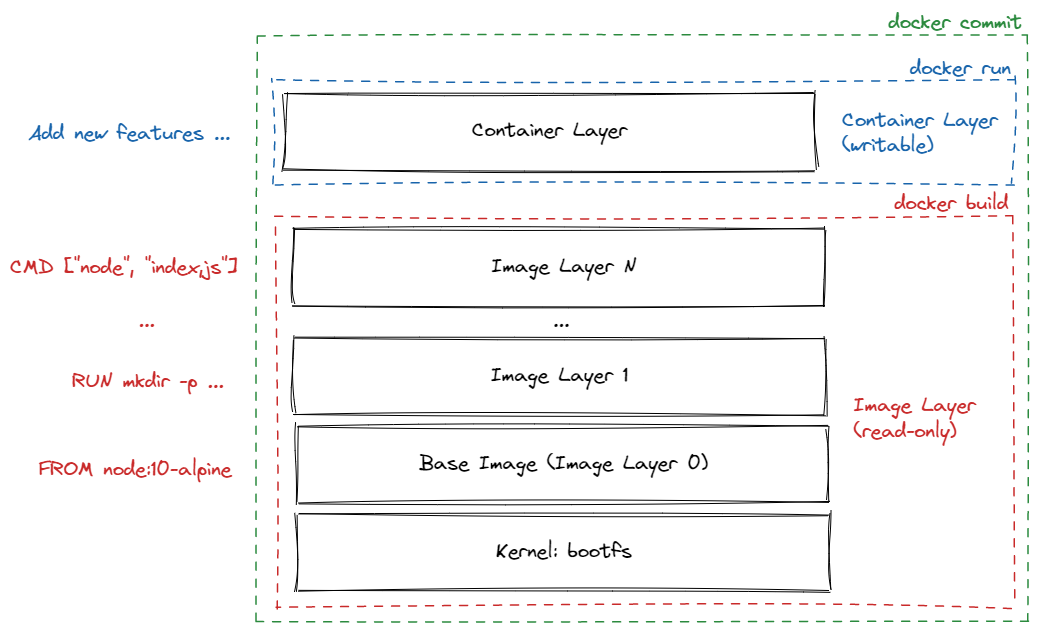
\includegraphics[width=350pt]{chapters/part-3/figures/dockerlayerdemo.png}
	\caption{A demonstration of docker image layer structure using the aforementioned example.} \label{ch:vac:fig:dockerlayerdemo}
\end{figure}

With the Dockerfile ready, use \verb|docker build| to build an image. An example is given as follows.
\begin{lstlisting}
$ docker build <path/url> -t <image name>
\end{lstlisting}
where \verb|<path/url>| is the path or URL to the directory where the Dockerfile locates (does not need to contain ``\verb|/Dockerfile|'' in its end), and \verb|-t| gives a tag, in this case an image name, to the image to build.

\subsection{Docker Image Management}

The most commonly used image operations can be categorized as follows.
\begin{itemize}
  \item Create an image.
  \item Create a container from an image.
  \item Upload and download an image from a remote server.
  \item Manage local images, such as listing down all images, deleting an image, etc.
\end{itemize}

The first two operations have been introduced in earlier sections. The third and last ones are introduced below. Use the following command to search for an image on the default remote repository server (Docker Hub).
\begin{lstlisting}
$ docker search <image name>
\end{lstlisting}
Use the following command to download or update an image from the default remote repository server as follows. Notice that different from \verb|docker run|, this command will not start a container from the image.
\begin{lstlisting}
$ docker pull <image name>
\end{lstlisting}
Notice that since images are stored by layers, if two images share common layers, it is unnecessary to pull the shared layers repeatedly when downloading the second image, if the first image already exists in the host machine. Command \verb|docker pull| is smart enough to automatically detect shared layers, and avoid duplicating download of layers.

Use the following commands to list down or remove images.
\begin{lstlisting}
$ docker image ls
$ docker image rm <image name>
$ docker image prune # remove all problematic images
$ docker image prune -a # remove all unused images
\end{lstlisting}
where \verb|prune| removes all problematic images, and \verb|prune -a| removes all unused images from local.

Use the following command to inspect an image, and list down its metadata details.
\begin{lstlisting}
$ docker image inspect <image name>
\end{lstlisting}

\section{Docker Hub}

Docker hub is a commonly used server for storing and sharing docker images. It is also the default remote repository server of docker engine. However, do notice that docker hub is not the only remote docker image server. Some alternatives are Amazon Elastic Container Registry, Red hat Quay, Azure Container Registry, Google Container Registry, etc.

After registering an account on docker bub, use the following command to login to the docker hub from your local machine.
\begin{lstlisting}
$ docker login --username=<user name>
Passowrd:
\end{lstlisting}

Assume that there is an image in the local machine, and an empty repository on docker hub. In order to push the local image to the docker hub, the first step is to add the remote repository and the ``\textit{RepoTags}'' in the local image as follows.
\begin{lstlisting}
$ docker tag <image name> <user name>/<repository name>:<version>
\end{lstlisting}
where \verb|<version>| is a tag usually used to distinguish the different branches or versions of the images on docker hub. For the first image upload, it can simply be \verb|latest|.

Use the following command to push the image to docker hub.
\begin{lstlisting}
$ docker push <user name>/<repository name>
\end{lstlisting}

\section{Portainer}

As introduced earlier, docker engine can be used to build and share images as well as start, monitor, and stop containers. It can be difficult for a user to manage containers manually when a lot of them are deployed. Container orchestrators such as Protainer and Kubernetes are helpful with managing containers. Many of these tools are able to automatically adjust the number of containers and balance their loads.

Portainer is an open-source container management tool. It has a web-based dashboard user interface. Notice that Portainer itself also runs in a container.

Before starting a Portainer container, it is a good practice to first create a docker volume for Portainer to store the database. Use the following command to create such docker volume.
\begin{lstlisting}
$ docker volume create portainer_data
\end{lstlisting}
Then run a Portainer container using
\begin{lstlisting}
$ docker run -d -p 8000:8000 -p 9000:9000 -p 9443:9443 --name portainer --restart=always -v /var/run/docker.sock:/var/run/docker.sock -v portainer_data:/data portainer/portainer-ce
\end{lstlisting}
where ports 8000, 9000 and 9443 are used for hosting HTTP traffic in development environments, hosting web interface, and hosting HTTPS or SSL-secured services, respectively. The \verb|docker.sock| is the socket that enables the docker server-side daemon to communicate with its command-line interface. The image name for Portainer community edition (distinguished form the business edition) is \verb|portainer/portainer-ce|.

Use \verb|https://localhost:9443| to login to the container. The following page in Fig. \ref{ch:vac:fig:portainerlogin} should pop up in the first-time login, asking the user to create and administration user.
\begin{figure}[htbp]
	\centering
	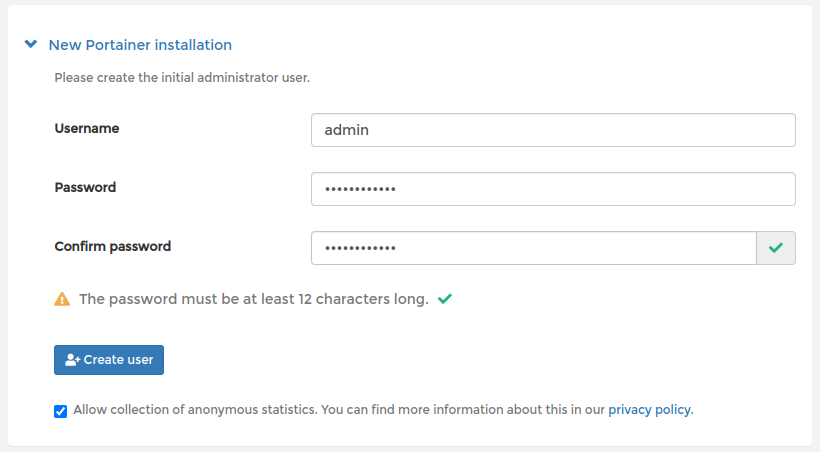
\includegraphics[width=350pt]{chapters/part-3/figures/portainerlogin.png}
	\caption{Portainer login page to create admin user.} \label{ch:vac:fig:portainerlogin}
\end{figure}

After creating the admin user and logging in, the status of images, containers and many more can be monitored via the dashboard, as shown in Figs. \ref{ch:vac:fig:portainerdashboard1}, \ref{ch:vac:fig:portainerdashboard2} and \ref{ch:vac:fig:portainerdashboard3}. Notice that in Fig. \ref{ch:vac:fig:portainerdashboard3}, using the ``quick action'' buttons, the user can check the specifics of the container and interact with its console, just like using \verb|docker container inspect| and \verb|docker exec|
\begin{figure}[htbp]
	\centering
	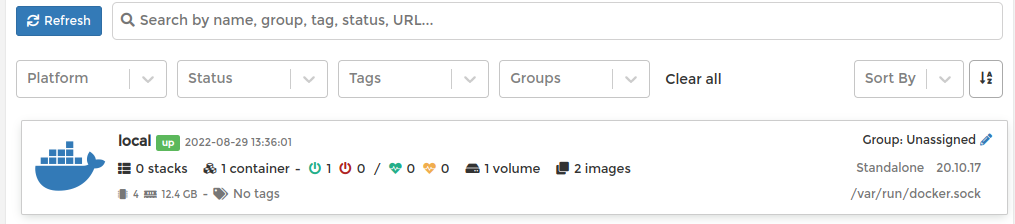
\includegraphics[width=350pt]{chapters/part-3/figures/portainerdashboard1.png}
	\caption{Portainer dashboard overview of docker servers.} \label{ch:vac:fig:portainerdashboard1}
\end{figure}

\begin{figure}[htbp]
	\centering
	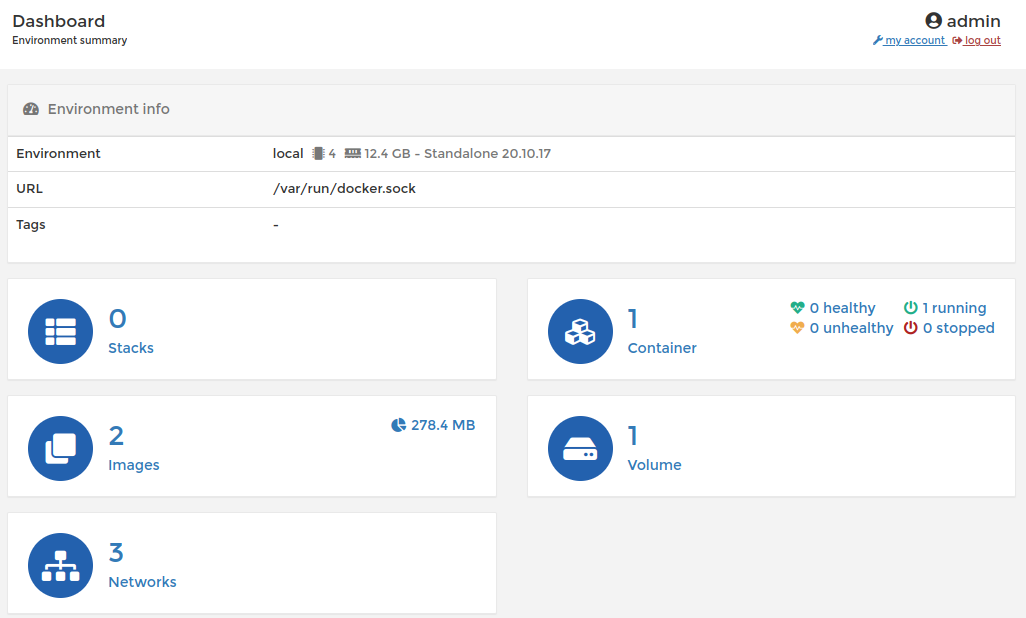
\includegraphics[width=350pt]{chapters/part-3/figures/portainerdashboard2.png}
	\caption{Portainer dashboard overview in a docker server.} \label{ch:vac:fig:portainerdashboard2}
\end{figure}

\begin{figure}[htbp]
	\centering
	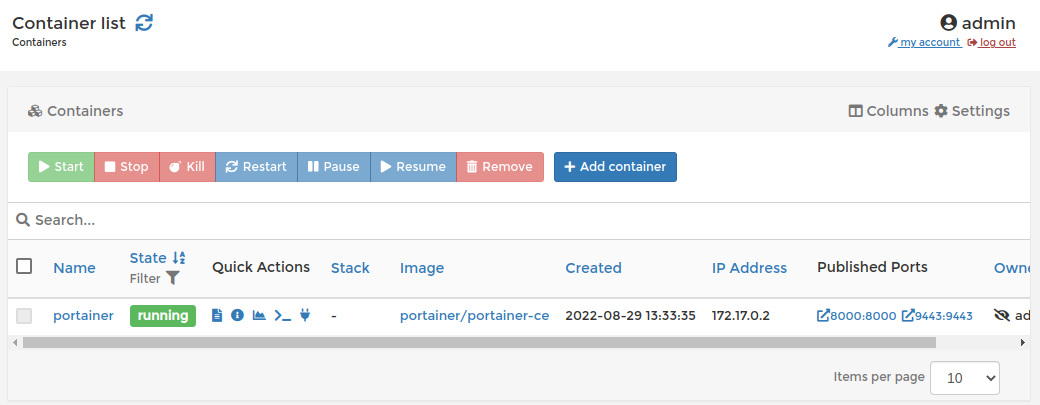
\includegraphics[width=350pt]{chapters/part-3/figures/portainerdashboard3.png}
	\caption{Portainer dashboard list down of all running containers.} \label{ch:vac:fig:portainerdashboard3}
\end{figure}

In summary, Portainer is an easy-to-use container management tool with clean graphical interface that a user can quickly get used to without a steep learning curve.



